\section{Introduction}

The cost of setting up a semiconductor foundry, also referred to 
as a \emph{fab}, 
has been increasing with technology scaling, and is 
currently upwards of \$5 billion~\cite{FoundryCost} for 
cutting-edge fabrication.
As a result, 
many semiconductor design companies have 
adopted the \textit{fabless} model, i.e., they outsource integrated circuit (IC) fabrication to one of a few large commercial IC foundries, often located off-shore. 
As per a recent study~\cite{}, 
four out of the 
top five semiconductor foundries by 
volume are located outside the United States. Most other countries  
either do not have a commercial 
foundry on-shore, and others that do only have access to low-end fabrication technology.  

The fabless model comes with the risk of compromising the 
designer's intellectual property (IP), i.e., the design of chip. 
When a designer outsources a chip for fabrication, the 
foundry obtains full access 
to the chip's layout (effectively a chip blue-print), 
from which it can 
recover its Boolean logic gate-level 
netlist and its 
Boolean 
functionality~\cite{rajendran2012security}.
%[Citation here? Shall we say IC extraction?]. 
An untrusted 
foundry can sell the designer's IP 
to its competitors or produce and sell extra copies of the 
chip. 
In many cases, the chip might implement proprietary 
protocols or algorithms --- the designer stands to loose competitive 
advantage if these are revealed to competing firms. 
[proprietary security protocol -- if revealed, security compromised?] 
[More citations to indicate that industry/DoD etc care about this?]~\cite{castillo2007ipp,kahng2001constraint,koushanfar2001hardware,musker1998protecting}  

%a heightened risk of intellectual property (IP) theft, 
%laws are lax  or weakly enforced. Hardware IP theft 

%However, this comes at the expense of trust. 
%How can the design company trust that the off-shore (untrusted) foundry has not {pirated its intellectual property} (IP), or maliciously modified the IC by inserting a hardware backdoor, commonly referred to as a {hardware Trojan}, in the chip? 
%Hardware IP theft and Trojan insertion have been recognized as 
%significant threats to the economic viability of outsourced 
%IC fabrication, and to the security of 
%ICs used in 
%areas such as
%critical infrastructure (for instance, communication networks, the smart grid and the emerging internet-of-things), national defense and consumer electronics. 

Logic locking, a technique first introduced by Roy et al.~\cite{roy2008epic}, 
is a promising solution to protect the designer's IP from 
being thieved by an untrusted foundry.\footnote{This technique has 
also been referred to as logic obfuscation~\cite{rajendran2012security} and logic encryption~\cite{dupuis2014novel,rajendran2012logic,rajendran2015fault} in the literature. However, following the lead of Roy et al., we will use the term logic locking throughout.}  
Logic locking works by inserting 
additional gates, referred to as \emph{key gates}, 
in a Boolean 
logic netlist with 
side-inputs that are referred to as \emph{key bits}. The key bits 
are 
stored in a key register. 
The netlist functions as intended \emph{only} 
for a certain key, and provides incorrect
outputs otherwise. 
The original logic locking procedure proposed by Roy et al. 
inserts XOR/XNOR gates at randomly chosen locations in the 
net-list. Subsequently, several other logic locking mechanisms have been proposed in literature that use different types of key gates or 
different procedures to insert key gates~\cite{rajendran2012security,rajendran2012logic,rajendran2015fault,plaza2015solving,dupuis2014novel,chakraborty2009harpoon}. 

The correct key, i.e., 
the key bits that produce the designer's intended 
functionality, 
is known to the designer but not to the foundry. The foundry manufactures the chip and ships the manufactured parts to the 
designer. The designer activates the chips by loading the 
correct key into the key register. 
The security of logic locking 
is premised on the foundry not knowing the correct key.
If the correct key is compromised, the foundry learns of the 
chip's functionality.\footnote{In fact, the protocol proposed by Roy et al. introduces two keys --- a master key that is common to each chip, and a per-instance chip key. See Section~\ref{sec:discussion} for more details? [how to word?]} 

  
Recent work by Subramanyan et al.~\cite{subramanyan2015evaluating} has 
established 
that all
of the logic locking techniques proposed in literature
are vulnerable to attack \emph{if} the 
untrusted foundry can obtain a 
working copy of the chip, i.e., 
a chip activated with the correct key. 
Note that the foundry cannot directly 
probe the activated chip for the key, but instead 
must infer it from 
the chip's input/output (IO) functionality.   
Subramanyan
et al.~\cite{subramanyan2015evaluating} propose an attack procedure that 
iteratively applies new inputs to the working chip and 
uses a SAT solver to 
(implicitly) eliminate incorrect keys. 
The procedure terminates when 
all but the correct key is [are?] eliminated. 
[too much detail?]
Subramanyan et al. show that procedure is 
remarkably effective in unlocking even large circuits locked 
with up to XXX keys [Number of keys is not explicitly mentioned in the paper]. Concurrently, El Massad et al.~\cite{el2015integrated} 
have proposed a similar attack on IC camouflaging, 
a different but conceptually related hardware 
defense mechanism.

\begin{figure*}
  \centering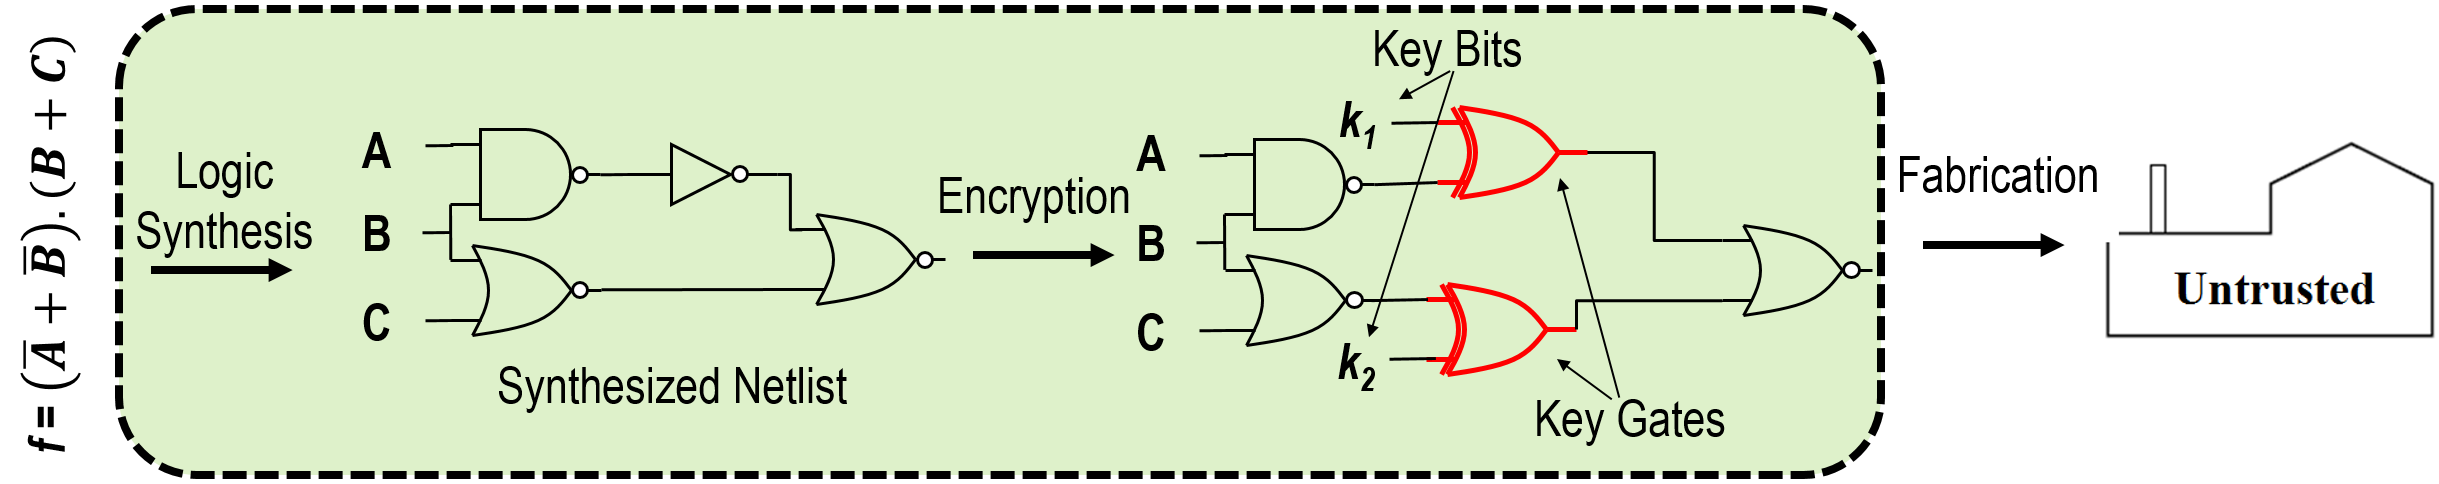
\includegraphics[width=.8\linewidth]{./figs/lenc-v1}
  \caption{The XOR logic locking scheme proposed by Roy et al.~\cite{roy2008epic}.}
  \label{fig:llock}
\end{figure*}


The work of 
Subramanyan et al.~\cite{subramanyan2015evaluating} and El-Massad et al.~\cite{el2015integrated} 
has established that 
existing logic 
locking mechanisms are insecure, but 
under \emph{conservative}  
assumptions on the attacker's capabilities.
That is, for the
attack to succeed, the attacker, i.e., the untrusted foundry fabricating the chip, 
must have access to a previously fabricated and 
activated copy of the chip.
Such a strong attack model 
is unrealistic in several scenarios of 
practical interest. 

%For one, the attack model above presupposes that the 
%chip has been previously fabricated. On the other hand, 
For one, a foundry is unlikely to 
be obtain working copies of 
chips fabricated by government agencies for 
critical infrastructure, defense and space applications 
since these are not available in the market.  
Second, even in the consumer electronics segment, a foundry 
has no access to working copies of
chips that are being fabricated for the first time. 
In fact, the first fabrication run is precisely 
when designer's 
might be most interested in using logic locking techniques to 
protect new and proprietary features introduced in the chip. 
%Finally, locking used to protect an algorithm/mechanisms that has no observable impact on I/O, but helps improve speed/performance. 

This leads to the following natural question: \emph{are existing 
logic locking mechanisms secure in the more 
practical setting in which the attacker only has access to the 
locked netlist?} The implicit answer to the question 
has in the literature been in the affirmative~\cite{roy2008epic}. 
%\emph{not} have access to a working chip. 
%[MEM: Has this been made explicit somewhere? If so, cite]
The first contribution of our work is 
to refute this implicit assumption. 
We show that netlists locked using 
existing mechanisms leak information about the key, even if the attacker does not have a working copy of the chip.
We demonstrate the vulnerability 
of existing logic locking mechanisms using a simple counter-example (see Section~\ref{}), and then by implementing a new attack 
procedure. We refer to this new attack as the
\emph{desynthesis attack}. 



Our attack builds on the observation that 
all existing 
logic mechanisms propose to insert key gates 
in a \emph{synthesized} 
Boolean logic netlist. 
Synthesis refers to 
the translation 
of a behavioural description of 
desired Boolean functionality, described for instance in 
a hardware description language (HDL) like Verilog, to a 
concrete implementation, a network 
of Boolean logic gates. Boolean logic is 
synthesized using 
commercial off-the-shelf synthesis tools. As with software 
compilers, synthesis tools output implementations with low 
cost, ideally the lowest cost. 
Herein lies the rub. For every incorrect key, 
there 
exists, in theory, a
different 
implementation with equal or lower cost, allowing 
lower cost keys to be eliminated. 
Section~\ref{sec:} describes a 
practical implementation of an attack built on the preceding 
observation. 
[DANGER: critic will say, how do you know which synthesis tool. 
Reply: there are only a few. Perhaps make this point in the 
discussion section.]


To address the security vulnerability exposed by the 
desynthesis attack,
we propose, in Section~\ref{sec:} 
a \emph{formal notion of security 
for logic locking} that 
guarantees that a locked netlist 
does not leak 
the correct key to the untrusted foundry.
To the 
best of our knowledge, this is the first time that 
a notion of security has been formalized for logic locking. 
Finally, we propose a new 
secure logic synthesis 
procedure, (NAME),   
that, given $f$, outputs a 
locked implementation  







%We design a new attack, which we refer to as a 
%\emph{desynthesis} attack, [.....]
%locked netlists leak information about the key.   



 
   





 
 






The rest of the paper is organized as follows. Section 3 
